\chapter{Methodology}

\section{Calculation of the Formation Energy of Defects in \CZTS}
See Lany paper + Keith's posted paper + encyclopoedia of defects paper \\

As discussed in section \ref{defects_in_PV}, defects in a solar absorber material can heavily impact on the performance of a photovoltaic device composed of that material. In this study we perform first principles calculations of two types of defects in the solar absorber material { \CZTS }. We firstly performed calculations of the formation energy of the charge neutral Cu-on-Zn and Zn-on-Cu anti-site defect pair, [$Cu_{Zn}^- + Zn_{Cu}^+$], in order to parameterize our Monte Carlo simulations of thermodynamic Cu-Zn disorder, which will be discussed further in section \ref{MC_section}. We also begin calculations of the formation energy of a sulfur vacancy in { \CZTS }. This defect can however take on three different charge states: $V_{S}^{0}$, $V_{S}^{+1}$ and $V_{S}^{+2}$, where electron occupancy varies from two to one to none respectively. We will then go on to calculate the formation energy as a function of the sulfur chemical potential to determine which charge state has the minimum formation energy at typical annealing conditions of { \CZTS }, in terms of temperature and pressure. This methodology is outlined in section \ref{defect_section}. However, special correction techniques must be applied when performing periodic calculations to simulate a bulk system with a finite unit cell when the unit cell possesses a net charge. This point is discussed in section \ref{supercell_section}.


\cite{defects_tutorial}



\subsection{Density Functional Theory \& Hybrid Functionals}\label{DFT_section}
Density functional theory (DFT) has been referred to as the most powerful method for assessing the properties of defects in materials \cite{defects_tutorial}. + refer to DFT in materials science paper?\\

The description of the electrons in a system requires the use of QM... outline of standard DFT...(explicitly introduce LDA and GGA)\\

\begin{itemize}
\item See Bechstedt book \cite{Bechstedt} + figures from Aron
\item discuss band gap underestimation in standard DFT (GGA mentioned during intro, also discuss GGA+U and limitations
\end{itemize}

DFT calculations typically yield reliable information about the atomic structure of defective systems, including relaxation of the host atoms. However the electronic structure has proved to be a greater challenge \cite{defects_tutorial}. Traditional functionals such as the LDA and GGA used in standard DFT, which were outlined above, severely underestimate band gaps of semiconductors and insulators, which then leads to large uncertainties in the position of defect levels. This issue can be addressed by going beyond standard DFT, such as by making use of many-body perturbation theory, where the GW approach is typically used \cite{defects_tutorial_19}. This method however is usually computationally expensive and difficult to implement self-consistently, so it is usually used to address the electronic structure only when used on top of atomic structures obtained from DFT \cite{defects_tutorial_20, defects_tutorial_21}, which is often denoted as DFT@G0W0 **CHECK** \cite{defects_tutorial}.

Hybrid functionals are another powerful way to overcome the limitations of standard DFT, they mix ... screened...
Hybrid functionals firstly have been round to produce band structures and band gaps in much better agreement with experiment, but also provide much more reliable description of charge localization, which is necessary to accurately model low symmetry defects or structures that give rise to polaron formation. Whereas standard DFT suffers from the self interaction error where ...
In particular, the screened hybrid functional of Heyd, Scuseria, and Ernzerhof (HSE) \cite{HSE} has proven reliable to predict formation energies and transition levels of native defects and impurities \cite{defects_tutorial}

Brief outline of hybrid DFT...


\subsection{The Supercell Method \& Corrections for Charged Defects}\label{supercell_section}
see Aron's lectures + DFT in materials science paper \cite{DFT_in_mat} + Lany paper\\

Another important advance has been the ability to cor-
rect for errors that arise from the use of supercells to describe charged defects. While these supercells can typically be made large enough to minimize interactions between a neu- tral defect and its mirror images, the long range of the Coulomb interaction renders this essentially impossible in the case of charged defects. Explicit correction schemes are therefore essential, and a supercell-size correction scheme based on the rigorous treatment of electrostatics was described in Refs. 31 and 32. \cite{defects_tutorial}


\subsection{Defect Formation Energy \& Equilibrium Concentration}\label{defect_section}
Show formula for defect formation E as a function of electronic and atomic chemical potentials, discuss chemical potentials (especially S!) and show Boltzmann expression for concentration.



\section{Monte Carlo Simulation of Thermodynamic Disorder in \CZTS}\label{MC_section}

\subsection{Mapping the Crystal Structure of { \CZTS } onto a Simple Lattice}

\begin{figure}[h!]
  \centering
    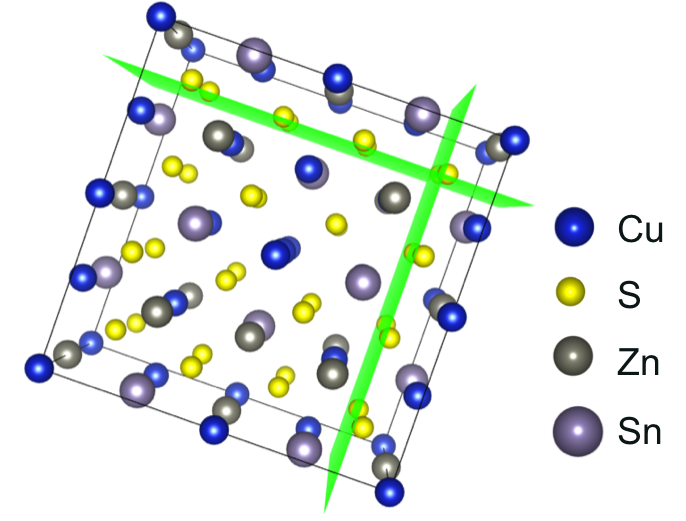
\includegraphics[width=0.5\textwidth]{figures/CZTS_lattice_mapping.png}
    \caption{A supercell of the perfect{ \CZTS } crystal lattice, which can be described by inter-penetrating face-centred cubic sub-lattices: one of metal cations and one of sulfur anions. Green planes are used as guides to the eye to show planes of S anions that form one of the two face-centred cubic sub-lattices.}
  \label{CZTS_lattice_mapping}
\end{figure}

In this study, we use a custom Monte Carlo code to simulate substitutional on-lattice disorder between Cu and Zn ions in {\CZTS } as a function of temperature. The crystal structure of {\CZTS } can be described by two inter-pentrating face-centred cubic (FCC) lattices: one of metal cations and one of sulfur anions, as shown in figure \ref{CZTS_lattice_mapping}. We consider the sulfur sub-lattice to be stationary because any substitution between ions in the cation sub-lattice and sulfur anion sub-lattice would be energetically infeasible and any substitutions amongst the sulfur anions in that sub-lattice would be energetically equivalent. The sulfur sub-lattice is therefore neglected during the Monte Carlo simulations but incorporated later in calculations of lattice electrostatics. This then reduces the problem of mapping the {\CZTS } crystal structure onto a simple lattice to just one FCC cation lattice. We then map this onto a simple cubic (SC) lattice for our simulations by introducing empty lattice sites into the SC lattice, as shown in figure \ref{eris_config_eg}. \\

\begin{figure}[h!]
  \centering
    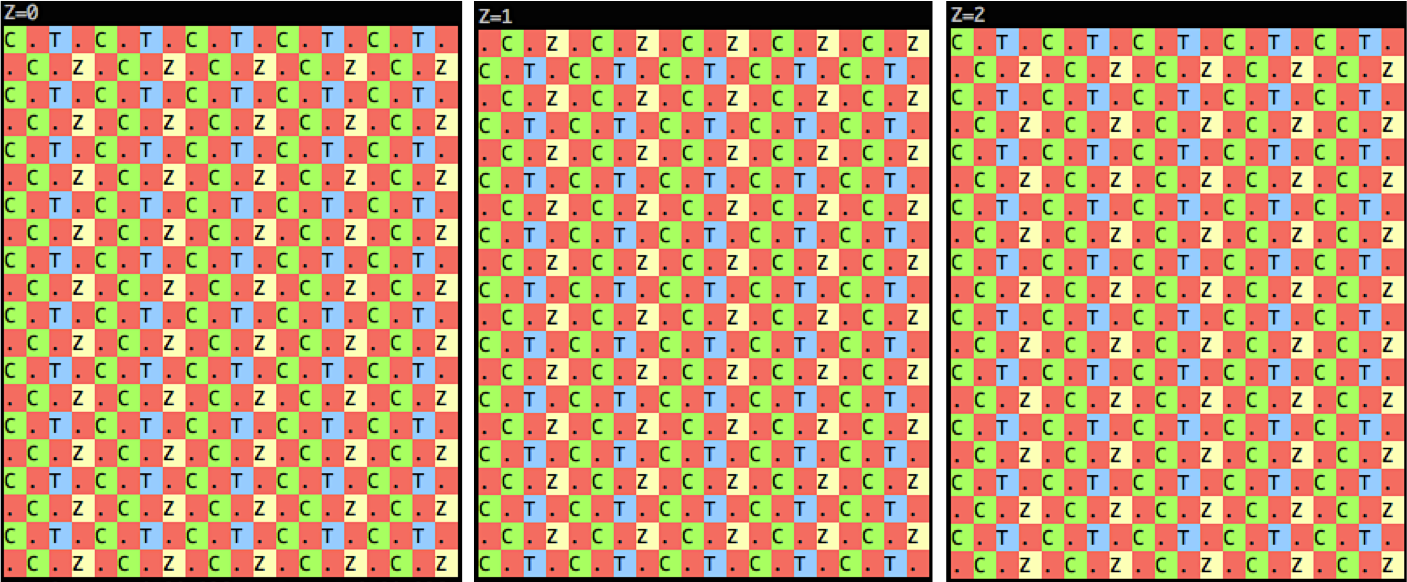
\includegraphics[width=0.95\textwidth]{figures/eris_config_eg.png}
    \caption{A two-dimensional (x-y) slice of a 20x20x20 cation sub-lattice of ordered { \CZTS }. Sulfur anions are neglected from the simulations and the face-centred cubic cation lattice is mapped onto a simple cubic lattice by including empty sites in the lattice. Alternating layers in the z-direction are displaced by one lattice unit in order to reproduce the correct kesterite structure. `C', `Z', `T' and `.' represent copper, zinc, tin and an empty site respectively.}
  \label{eris_config_eg}
\end{figure}

For some of our simulations, we initialise the system as the perfectly ordered crystal structure of CZTS. Then for simulations where we want to start from a disordered system, we again take this perfectly ordered initial structure but 'shuffle` Cu and Zn ions. An initial configuration of a large SC lattice of perfectly ordered CZTS is generated by producing a supercell of a unit cell of the perfectly ordered structure, where this unit cell was determined by examining the geometry of CZTS one layer at a time in three dimensions. An example of this analysis is shown in figure \ref{unit_cell_eris_supercell}. The smallest unit cell was found to be a 2x2x4 cell when including the gap sites. The crystal structure of {\CZTS } can also be described by alternating layers of Cu-Zn and Cu-Sn \cite{Schorr}, as shown in figure \ref{CZTS_cell}. For the unit cells generated by eris, this corresponds to when the system is viewed along the y-axis and as we fix Sn ions in our simulations, we would expect this direction to always have this same repeating pattern when the system is perfectly ordered. We therefore intend to use order in this direction as one of our order parameters, which is discussed further in section \ref{RDF_methods}. However, we will also check that our system crystallises in the same direction as we would expect it to by performing simulations from an initial randomized configuration until the ground state crystal structure is recovered at low temperatures. This process will be discussed in the results section.\\

\begin{figure}[h!]
  \centering
    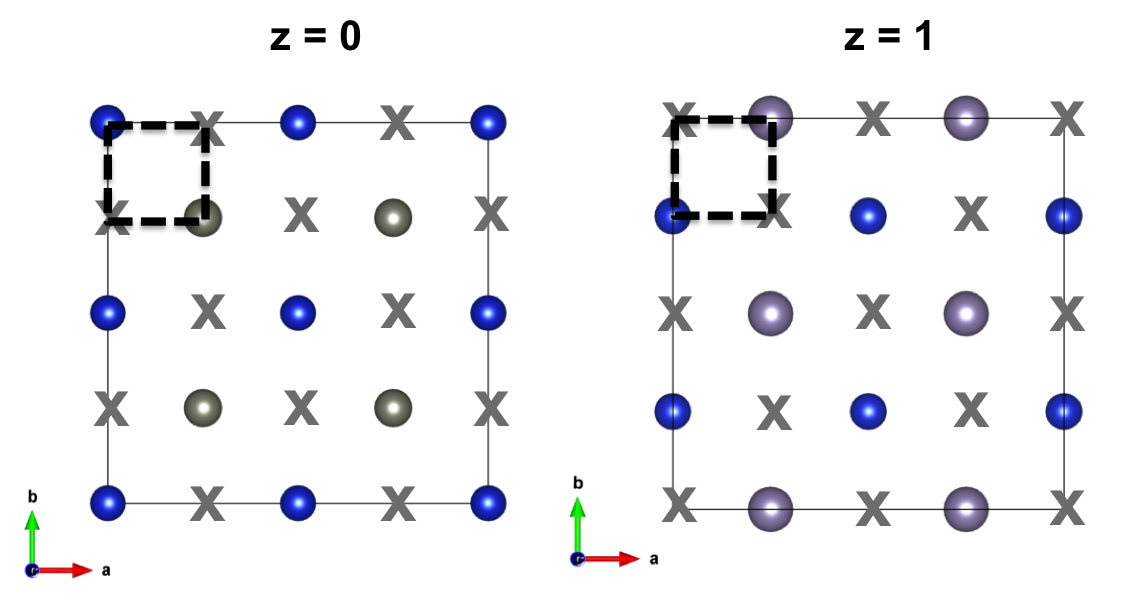
\includegraphics[width=0.9\textwidth]{figures/unit_cell_eris_supercell.png}
    \caption{Some of the single layers of a CZTS supercell used to determine the minimum cation unit cell for constructing supercells in on-lattice Monte Carlo simulations. Here crosses are used to denote the empty sites used in to map a face-centred cubic lattice onto a simple cubic lattice.}
  \label{unit_cell_eris_supercell}
\end{figure}

%We therefore fill the lattice in this way in a checkerboard-like fashion when constructing a perfectly ordered on-lattice representation of the crystal structure, 2D slices of the ordered system are shown in figure \ref{eris_config_eg}. 

During our simulation the separation between lattice sites is one lattice unit but this is re-scaled for calculations of lattice electrostatics using our DFT-optimised lattice parameters of $\frac{a}{2}  = \frac{b}{2} = \frac{5.44}{2} \AA$. Where the lattice parameters are divided by 2 as empty sites are placed in between ions to map the FCC structure onto an SC lattice. Figure \ref{CZTS_lattice_scaling} shows flat representations of the crystal structure, with empty lattice sites marked out by crosses. Lattice parameter c for our model will then be approximated to 2a, which is very close to the DFT-optimised value of 10.86 \AA .  

\begin{figure}[h!]
  \centering
    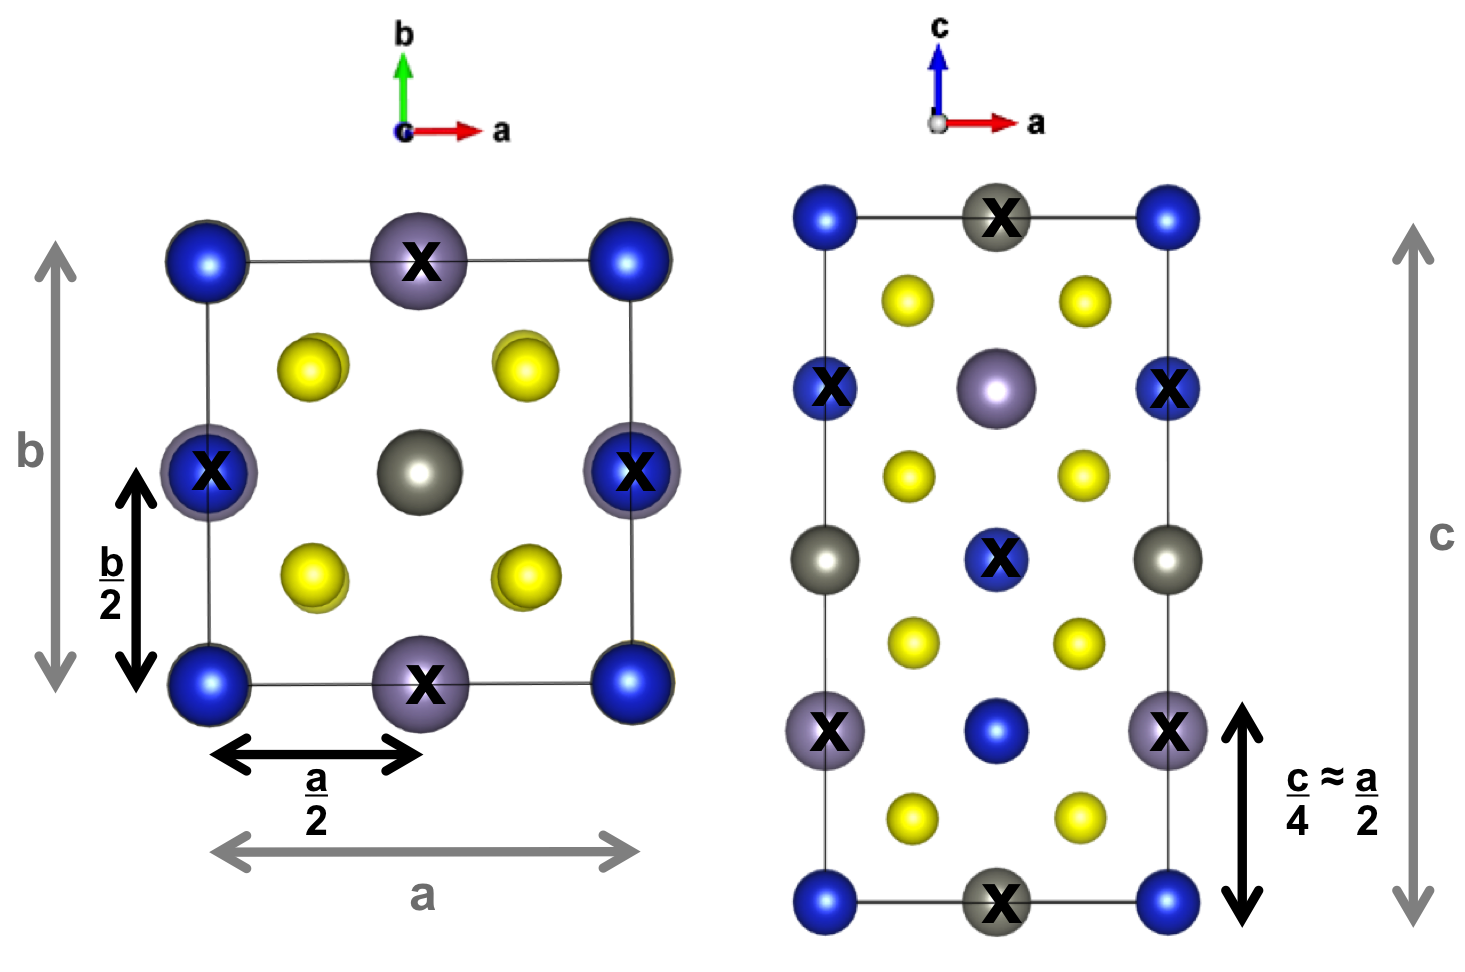
\includegraphics[width=0.9\textwidth]{figures/CZTS_lattice_scaling.png}
    \caption{Visuals of the { \CZTS } crystal structure showing positions of empty sites (denoted by x's) used to map the face-centred cubic lattice of the cations onto a simple cubic lattice. Lattice parameters obtained from hybrid density functional theory geometry optimizations are a = b = 5.43770 \AA and c = 10.85670 \AA, and so c is approximately 2a.}
  \label{CZTS_lattice_scaling}
\end{figure}


\subsection{Monte Carlo Simulation with the Metropolis Algorithm}

The Monte Carlo method can be used to calculate thermodynamic information about a system of N interacting ions represented on a 3D lattice by using classical statistics, considering only two-body forces and assuming that the potential field of an ion is spherically symmetric. If we know the positions of the N interacting ions on the lattice then the potential energy of the system can be calculated using equation \ref{pot_E}, where V is the Coulombic potential between two ions and $d_{ij}$ is the minimum distance between ions i and j \cite{Metropolis}.
\begin{equation}\label{pot_E}
E = \frac{1}{2} \sum_{i=1}^N \sum_{j=1}^N V d_{ij}
\end{equation}
To calculate the properties of the system, the canonical ensemble is used where the temperature, number of ions and volume are all constant. In this ensemble, the equilibrium value for any quantity of interest, B, is given by equation \ref{av}, where $E_\alpha$ is the energy of the system when in state $\alpha$ and $p_\alpha$ is the probability of the system being in state $\alpha$.
\begin{equation}\label{av}
<B> = \frac{ \sum_\alpha e^{-\frac{E_\alpha}{k_bT}} B_\alpha}{ \sum_\alpha e^{-\frac{E_\alpha}{k_bT}}} = \frac{ \sum_\alpha e^{-\frac{E_\alpha}{k_bT}} B_\alpha}{Q} = \sum_\alpha B_\alpha p_\alpha
\end{equation}
\begin{equation}\label{prob}
p_\alpha = \frac{  e^{-\frac{E_\alpha}{k_bT}} }{ \sum_{\alpha} e^{-\frac{E_\alpha}{k_bT}}} =\frac{  e^{-\frac{E_\alpha}{k_bT}} }{Q}
\end{equation}
Q in equation \ref{av} is called the partition function. For most systems calculating the value of the partition function requires the summation over a large number of states. When applying the Monte Carlo method to a system of particles, the summation over discrete states for Q is replaced by a set of integrals. This is shown in equation \ref{MC_av} where $U(\mathbf{r}^N)$ is the potential energy of the system which depends upon the position, \textbf{r}, of the N interacting ions in the system and $Z_{NVT}$ is the configurational integral \cite{Lesar3}.
%\begin{equation}\label{MC_prob}
%p(\mathbf{r}^N) = \frac{  e^{-\frac{U(\mathbf{r}^N)}{k_bT}} }{\int %e^{-\frac{U(\mathbf{r}^N)}{k_bT}} d\mathbf{r}^N}  = \frac{  e^{-\frac{U(\mathbf{r}^N)}%{k_bT}}}{Z_{NVT}} 
%\end{equation}
\begin{equation}\label{MC_av}
<U> = \frac{ \int e^{-\frac{U(\mathbf{r}^N)}{k_bT}} U(\mathbf{r}^N) d\mathbf{r}^N}{\int e^{-\frac{U(\mathbf{r}^N)}{k_bT}} d\mathbf{r}^N}  = \frac{  \int e^{-\frac{U(\mathbf{r}^N)}{k_bT}} U(\mathbf{r}^N) d\mathbf{r}^N}{Z_{NVT}} 
\end{equation}
The configurational integral is over the three coordinates of each ion, as shown in equation \ref{dr}. There are therefore 3N coordinates that define all possible configurations of the system.
\begin{equation}d \mathbf{r}^N = dx_1 dy_1 dz_1 dx_2 dy_2 dz_2... dx_N dy_N dz_N\end{equation}\label{dr}
For a system containing several hundred ions this would be a several-hundred dimensional integral over the configuration space, which would be impractical to carry out by the usual numerical methods. The Monte Carlo method for many-dimensional integrals is used for this purpose \cite{Metropolis}. It is conceptually easiest to think about this method for a one-dimensional integral. This method involves sampling a large number of random points within a region defined by the limits of the integral. The integrated function is then the fraction of points that fall below the curve of the function multiplied by the area of the sampled region. The value obtained becomes a better approximation to the actual value of the integral as the number of random numbers, called Monte Carlo steps (MCS), used to sample the integration region increases. \cite{Lesar3}.

The Standard Monte Carlo method for our system would involve placing each of the N ions at random positions in the lattice to define a random point in the 3N-dimensional configuration space. The energy of the system would then be calculated using equation \ref{pot_E} and the configuration would then be weighted using $e^{-\frac{U(\mathbf{r}^N)}{k_bT}}$ when obtaining the equilibrium value of U. However, many configurations are very improbable so performing this calculation for every possible configuration would be inefficient and unnecessary to sufficiently evaluate the ensemble. The custom Monte Carlo code in this study makes use of the Metropolis modified Monte Carlo scheme \cite{Metropolis}. In this implementation of the Monte Carlo method, instead of choosing configurations randomly and then weighting them, the Metropolis algorithm considers the relative probability of a system being in a new configuration, $\beta$, to that of being in the current configuration, $\alpha$. This is shown in equation \ref{relative_prob}, where $E_\alpha$ is the energy of state $\alpha$ and $E_\beta$ is the energy of state $\beta$.
\begin{equation}\label{relative_prob}
\frac{p_\beta}{p_\alpha} = \frac{  e^{-\frac{E_\alpha}{k_bT}} }{Q} \frac{Q}{  e^{-\frac{E_\alpha}{k_bT}} } = e^{- \frac{E_\beta - E_\alpha}{k_BT}}
\end{equation}
The relative probabilities of the two states are completely determined by the energy 
difference, such that if:
\begin{equation}\label{met}
\Delta E = E_{\beta} - E_{\alpha} \leq 0 \text{   then   } \frac{p_{\beta}}{p_{\alpha}} \geq 1 
\end{equation}
and if
\begin{equation}\label{met2}
\Delta E = E_{\beta} - E_{\alpha} > 0 \text{   then   } \frac{p_{\beta}}{p_{\alpha}} < 1
\end{equation}

The Metropolis algorithm creates a list of configurations through configuration space that has the correct probability distribution. This list is called a trajectory through configuration space. The approach involves making a trial move of the system to a new configuration, in the case of our study this would be a substitution between a Cu and a Zn ion. It is then decided if this new configuration should be added to the trajectory or not based on the probability of the new configuration relative to the current configuration. If the relative probability is  $\geq$ 1, as shown in equation \ref{met}, then the move is accepted and added to the trajectory. However, if the relative probability is $<$ 1 then the move will only be accepted if $e^{-\frac{\Delta E}{k_BT}} \ge$ a random number generated between 0 and 1 \cite{Lesar3}.


\subsection{Equilibration \& Finite Size Effects}
Our Monte Carlo model for Cu-Zn disorder is analogous to the Ising model of a magnet, descriptions of which can be found in many textbooks such as references \citenum{MC} and \citenum{MC_Landau}. In the case of an Ising model, the trial moves in the Metropolis algorithm are spin flips, whereas in our model the trial moves are swaps between Cu and Zn ions. In the case of the Ising model it is usually the average magnetization of the system or internal energy as a function of temperature that are the quantities of interest. In our system, it is the distribution of the electrostatic potential across the system that is of interest, as this can be related to the observed band tailing. We are also interested in the corresponding configuration of the ions (and extent of disorder) that results in such a distribution. In the case of the Ising model when, for example, determining the magnetization of a system at a given temperature, the simulation must be run for a suitably long time until the system has come to equilibrium at that temperature. This is referred to as the equilibration time and the point at which a system has attained equilibrium can be defined as being when the average probability of finding the system in any particular state $\alpha$ is proportional to the Boltzmann weight of that state, $e^{-\frac{E_\alpha}{k_bT}}$. Once the system has equilibrated, the quantity of interest such as the magnetization must then be again measured over a suitably long time and averaged \cite{MC}.

To gauge if a system has reached equilibrium, in the case of the Ising model, it is common practice to run the simulation for a large number of Monte Carlo steps (MCS) (where one MCS corresponds to attempting a trial spin-flip at all sites in the system once) and looking for how the value of a quantity of interest, such as the average magnetization across the system, changes with increasing number of MCS as the simulation progresses. Equilibration is often considered as the point at which the value of a quantity of interest, which initially changes by a large amount, eventually converges to fluctuating about a steady average value. An example of this is shown in figure \ref{ising_equil}a. This is dependent upon the principle that a system in equilibrium spends the overwhelming majority of its time in a small subset of states in which its properties take a narrow range of values \cite{MC}. In the case of our system, it is the distribution in electrostatic potential across the system that is of interest so we will look for a point after which the variance of the distribution of electrostatic potentials across the system has reached a steady value.

\begin{figure}[h!]
  \centering
    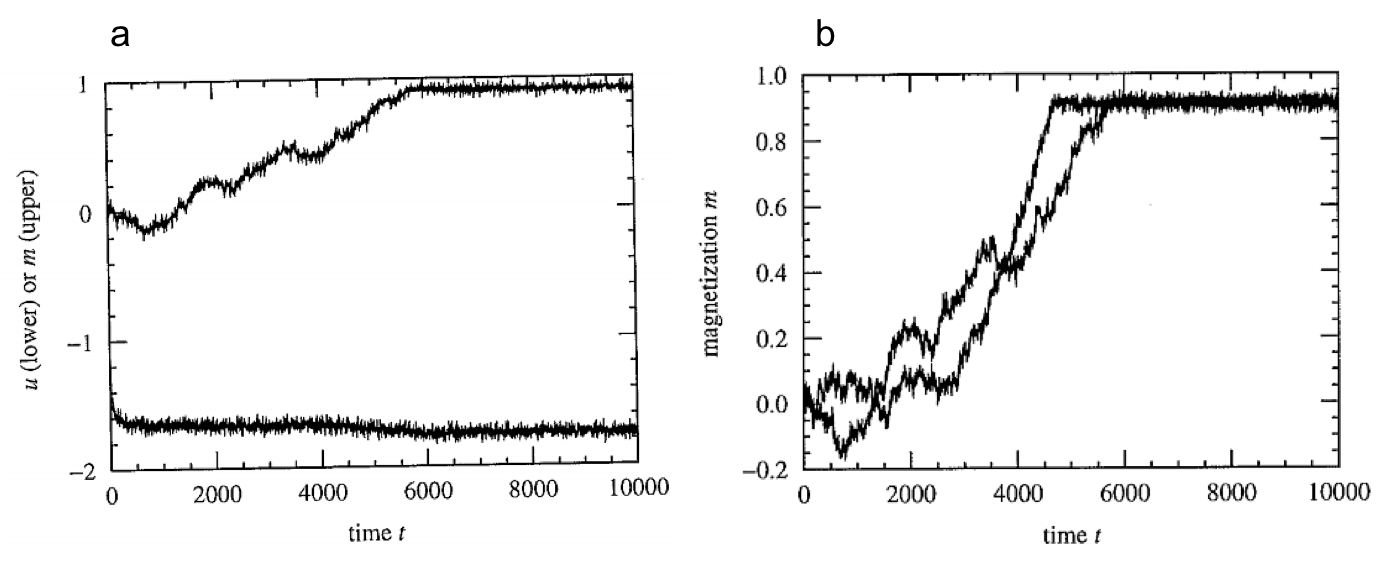
\includegraphics[width=0.9\textwidth]{figures/ising_equil.png}
    \caption{The magnetization (upper curve) and internal energy (lower curve) per site of a two-dimensional Ising model simulated using the Metropolis algorithm (a). Magnetization as a function of time for two different simulations (b). Time is measured in Monte Carlo steps per lattice site. Figures taken from \citenum{MC}.}
  \label{ising_equil}
\end{figure}

Provided the simulation is allowed to run for a sufficiently long time to reach this minimum configuration, the final configuration for a given system at a given temperature should always be the same, this point is illustrated in figure \ref{ising_equil}b. However,  as this is a stochastic method, making use of sampling many times with random numbers in order to determine the minimum energy configuration of the system, the trajectory to reach this final configuration will by nature be random and so we can draw no conclusions from configurations of the system until the final configuration at the particular temperature is reached. Even then we must consider the possibility of our system finding local minima instead of global minima, and therefore giving a false impression of having equilibrated. For this reason we perform multiple runs of the simulations, each seeded with different random numbers to ensure that the same final configurations, and associated equilibrium properties, are obtained. 

As simulations are performed for finite lattices, in order to simulate a bulk system the edges or `boundaries' of the system must be treated carefully. The boundaries can be effectively eliminated through the use of periodic boundary conditions (PBCs). In the case of an Ising model, this means that the first spin in a row interacts with the last spin in the row as if it were a nearest neighbour, and vice versa \cite{MC_Landau}. This principle is illustrated in figure \ref{MC_PBCs}. Although this procedure effectively eliminates boundary effects, the system is still characterized by the finite lattice size, L, which limits the correlation length to $\frac{L}{2}$. Resultant properties of the system may then differ for the bulk system than for the simulated system. We therefore perform simulations with increasing system size to look for any differences in the quantities of interest.

\begin{figure}[h!]
  \centering
    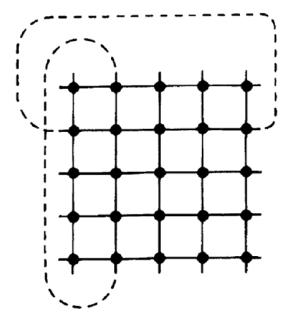
\includegraphics[width=0.4\textwidth]{figures/MC_PBCs.png}
    \caption{Typical periodic boundary conditions for the two-dimensional Ising model. Figure taken from \citenum{MC_Landau}.}
  \label{MC_PBCs}
\end{figure}

\subsection{Multi-Scale Approach with Density Functional Theory}
\begin{equation}\label{eris_interaction}
E_{electrostatic} = \frac{q_1q_2}{4\pi\epsilon_0\epsilon_r}e^2\frac{1}{r} = q_1q_2 I_{electrostatic}
\end{equation}
Equation \ref{eris_interaction} can be used to calculate the electrostatic interaction between a pairs of ions, where $q_1$ and $q_2$ are the bare formal charges, r is the separation of the point charges and $\epsilon_r$ is the bulk static relative dielectric constant. The interaction between all pairs of ions within the system are summed over when calculating the change in the energy of the system after performing a trial move in our Monte Carlo simulations.
We separate out the parameter $I_{electrostatic}$ in our simulations. The value is first calculated considering a purely classical, electrostatic case where only the bare formal charges on the ions are considered and the bulk dielectric constant of { \CZTS } is used. Using a value of 13.2 for $\epsilon_r$ and 3.8 $\AA$ for r, which is the separation of nearest-neighbour Cu-Zn ions, gives a value of -0.284 eV for $I_{electrostatic}$.
This treatment however only accounts for the Coulombic interaction between the point charges and neglects any changes in the electronic structure during defect formation. The screening effect of the electronic structure would be more significant for the microscopic dielectric constant than for the bulk, macroscopic dielectric constant.
In this study therefore we scale the interaction energy, $I_{interaction}$, in the simulations by comparing the formation energy of a nearest-neighbour Cu-Zn anti-site defect pair calculated using the classical code GULP to that obtained using quantum mechanical hybrid-density functional theory and the VASP code, where effects of the electronic structure are included in the calculation. We found that the defect formation energy obtained using VASP was approximately 1.5 times that obtained with GULP, we therefore scaled the interaction energy by the same amount and so $I_{DFT} = 1.5 \times I_{electrostatic} = - 0.425$ eV. Through doing this we aim to scale the macroscopic dielectric constant to be closer to the value of the microscopic dielectric constant.




\subsection{Quantification of Disorder Using Radial Distribution Functions}\label{RDF_methods}
\begin{itemize}
\item Brief overview of what an RDF is
\item See new lab book and make figures to explain
\item Reproducing GS: Cu-Zn RDF first peak to describe Cu Zn Cu layer, Cu-Sn RDF first peak to describe Cu Sn Cu layer nearest neighbours
\item Using RDFs from initial, perfectly ordered system as a reference point: Cu-Sn and Cu-Zn perfectly overlayed, but expect to separate with disorder. First peak (near-neighbours) for Cu-Sn should remain same as Sn is fixed, but Cu-Zn first peak will change as will subsequent peaks for both.
\item Need to normalize to recover coordination number for first peak?
\item Increasing intensity of new nearest neighbour Cu-Cu and Zn-Zn peaks for disordered systems with increasing disorder
\end{itemize}


\subsection{Band Tailing from the Distribution of Electrostatic Potential}
May later move this to further work so methodology not necessary? + need to alter end of intro section on CZTS performance bottlenecks




\section{Calculation of Intrinsic Band Gap Broadening in \CZTS}
Discuss MAPI paper, calculating contribution to broadening from acoustic lattice vibrations, explicitly discuss calculations of elastic constant and deformation potential.


\section{Calculation of Optoelectronic Properties of Candidate Solar Absorber Materials}\label{properties_methods}
\begin{itemize}
\item Hybrid geometry optimization with lattice fixed (but ions allowed to relax), starting from high quality XRD data and our own for stephanite performed by Prof Mark Weller (refer to original sources)
\item Hybrid band structure calculations with FHI-aims
\item Calculation of effective masses?
\end{itemize}

See MRes project2 write up + read up on SLME analysis and discuss this? Or discuss this just in further work?

                            